\documentclass[9pt,addpoints]{exam}
\usepackage{enumitem}
\usepackage{amsfonts,amssymb,amsmath, amsthm}
\usepackage{graphicx}
\usepackage{systeme}
\usepackage{pgf,tikz,pgfplots}
\pgfplotsset{compat=1.15}
\usepgfplotslibrary{fillbetween}
\usepackage{mathrsfs}
\usetikzlibrary{arrows}
\usetikzlibrary{calc}
\pagestyle{headandfoot}
%\firstpageheadrule
\runningheader{Homework 1}{}{Page \thepage\ of \numpages}
\runningheadrule
\author{Aaron GK}
\usepackage{geometry}
\geometry{
	a4paper,
	total={170mm,257mm},
	left=10mm,
	right=10mm,
	bottom=5mm,
	top=5mm,
}
\firstpagefooter{}{}{}
\runningfooter{}{}{}


\begin{document}
	\title{St John Baptist De La Salle Catholic School, Addis Ababa\\
		\large Homework 1 \\
		2nd Quarter}
	\maketitle
	\begin{center}
		\fbox{\fbox{\parbox{6in}{\centering
					Notes, and use of other aids is allowed.  Read all directions carefully and write your answers in the space provided.  To receive full credit, you must show all of your work. \textbf{Cheating or indications of cheating and similar answers will be punished accordingly}. 
		}}}
		\subsubsection*{Information}
		\begin{itemize}
			\item The homework is due on \textbf{Monday}, \textbf{December 5th}.
			\item You should Work on it \textbf{individually} and consult me if you have any questions. As I have reiterated multiple times, cheating will have a serious consequence.
			\item For purposes of neatness and simplicity of grading, you should do the homework on an \textbf{A-4 paper}.
		\end{itemize}
	\end{center}
	\begin{center}
		\subsection*{Questions}
	\end{center}

	\begin{questions}
			\subsubsection*{Conceptual Problems}
		\question We do have a great deal of relationship between rotational and translational physical quantities. List the translational equivalents for the following rotational physical quantities: \textit{torque, angular momentum, moment of inertia} and \textit{angular impulse}.
		\question When there is a global heating trend on Earth, the atmosphere expands and the length of the day increases very slightly. Explain why the length of a day increases.
		\question A point mass is going down an inclined plane. It also rotates while going down the inclined plane - we can deduce that the point mass has both a \textbf{translational}(\textit{linear}) and \textbf{rotational} kinetic energy. What percentage of the total kinetic energy is the rotational kinetic energy? (Assume the moment of inertia of a point mass is $\text{mr}^2$)
		\question A uniform 4.0-m plank weighing 200.0 N rests against the corner of a wall, as shown below. There is no friction at the point where the plank meets the corner. (a) Find the forces that the corner and the floor exert on the plank. (b) What is the minimum coefficient of static friction between the floor and the plank to prevent the plank from slipping?
		\begin{center}
					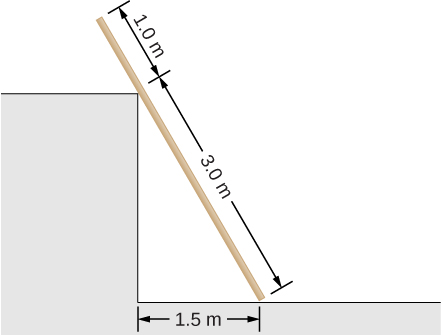
\includegraphics[scale=0.8]{ladder.jpeg}
		\end{center}
		\question A constant torque is applied to a rotating object whose moment of inertia is  16 kgm$^2$ around the axis of rotation. If the body starts from rest and attains an angular velocity of 20.0 rad/s in 10.0 s, what is the applied torque?
		\question On a planet whose radius is  1.2$\times10^{10}$m, the acceleration due to gravity at the surface of the planet is  15m/s$^2$. What is the mass of the planet?
		\question Eros has an elliptical orbit about the Sun, with a perihelion distance of 1.13 AU and aphelion distance of 1.78 AU. What is the period of its orbit? (1 AU = 1.496$\times10^8$km)
		\question A centrifuge at Addis Ababa University has a radius of 8.0 m and can produce forces on its payload of 18 \textit{g}s or 18 times the force of gravity on  the surface of the Earth. (a) What is the angular momentum of a 20-kg payload that experiences 10 gs in the centrifuge? (b) If the driver motor was turned off in (a) and the payload lost 10 kg, what would be its new spin rate, taking into account there are no frictional forces present?
		
	\end{questions}		
\end{document}